\section{Технологическая часть}

\subsection{Выбор СУБД}

В таблице \ref{tab:subd} произведено сравнение наиболее популярных СУБД, которые могут быть использованы для реализации хранения данных в разрабатываемом программном продукте.

\begin{table}[!h]
	\captionsetup{justification=centering}
	\caption{\label{tab:subd} Особенности различных СУБД}
	\begin{center}
		\begin{tabular}{|p{0.15\textwidth}|p{0.2\textwidth}|p{0.15\textwidth}|p{0.15\textwidth}|p{0.15\textwidth}|}
			\hline
			\textbf{Особенность} & \textbf{MySQL} & \textbf{PostgreSQL} & \textbf{MS SQL Server} & \textbf{Oracle Database} \\
			\hline
			Open source & GNU GPL с открытым исходным кодом & Открытый исходный код & Коммерческая & Коммерческая\\
			\hline
			Соответствие ACID & Частичное (зависит от версии) \cite{acid} & Полное & Полное & Полное\\
			\hline
			NoSQL / JSON & Поддержка некоторых функций & JSON, NoSQL & JSON, NoSQL & JSON, NoSQL\\
			\hline
			Поддержка MERGE & Да & Нет & Да & Да\\
			\hline
		\end{tabular}
	\end{center}
\end{table}

Таким образом, для реализации проекта в качестве СУБД будет использоваться PostgreSQL, так как он является свободно распространяемым и удовлетворяет всем необходимым требованиям в рамках поставленной задачи.

\subsection{Выбор ЯП и среды программирования}

Для реализации проекта в качестве языка программирования был выбран язык Python, так как:
\begin{itemize}
	\item этот язык поддерживает работу с PostgreSQL (в моём случае для этого будет использоваться библиотека psycopg2);
	\item данный язык является полностью объектно-ориентированным (всё является объектами) \cite{python}, что позволяет в полной мере использовать классы при написании программы;
	\item в этом языке присутствует PyQt (набор расширений графического фреймворка Qt для языка программирования Python, выполненный в виде расширения Python \cite{pyqt}), позволяющий легко создавать графический интерфейс для приложения.
\end{itemize}

В качестве среды разработки был выбран PyCharm по следующим причинам:
\begin{itemize}
	\item наличие бесплатной версии Community Edition;
	\item множество удобств, облегчающих процесс написания и отладки кода.
\end{itemize}

\subsection{Детали реализации}
В приложениях А -- Б представлен пример реализации frontend части приложения.

В приложении В представлена реализация соединения с базой данных в соответствии с ролевой моделью.

Помимо этого, на уровне базы данных была реализована процедура, необходимая для удаления реп. базы (приложения Г – Д).

%\subsection{Интерфейс программы}

На рисунках ниже представлен основной интерфейс приложения.

\begin{figure}[h!]
	\begin{center}
		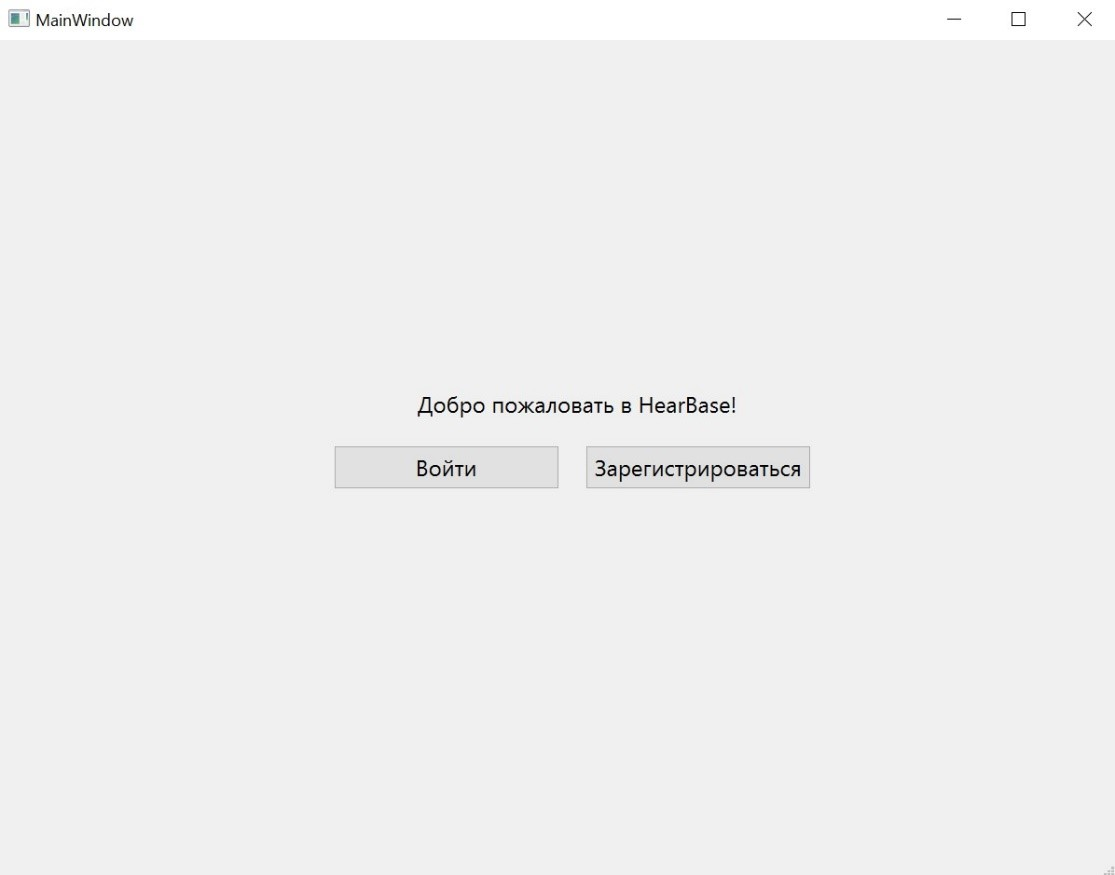
\includegraphics[scale=1]{jpg/Welcome.jpg}
	\end{center}
	\captionsetup{justification=centering}
	\caption{Окно с приглашением}
\end{figure}

\newpage

\begin{figure}[h!]
	\begin{center}
		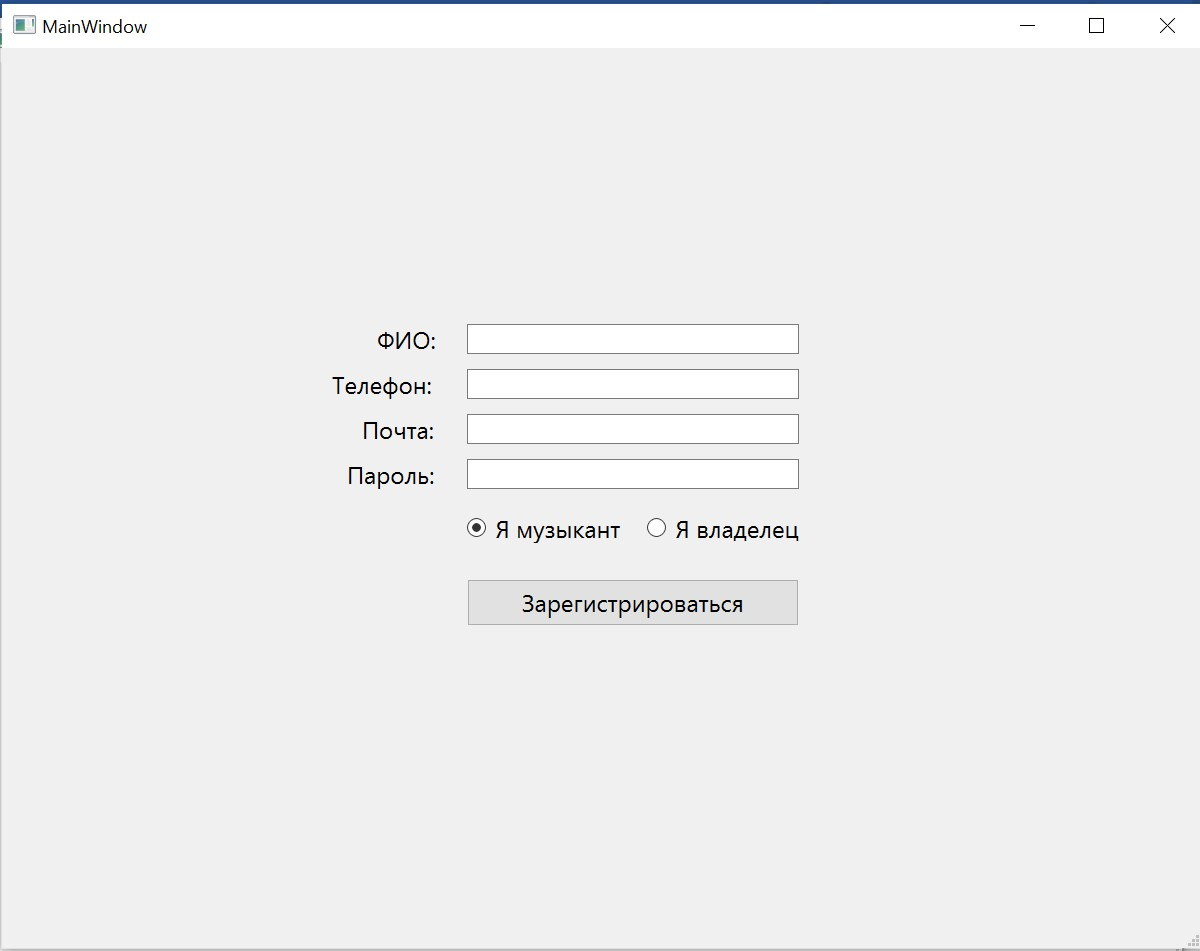
\includegraphics[scale=0.4]{jpg/Reg.jpg}
	\end{center}
	\captionsetup{justification=centering}
	\caption{Окно регистрации}
\end{figure}

\begin{figure}[h!]
	\begin{center}
		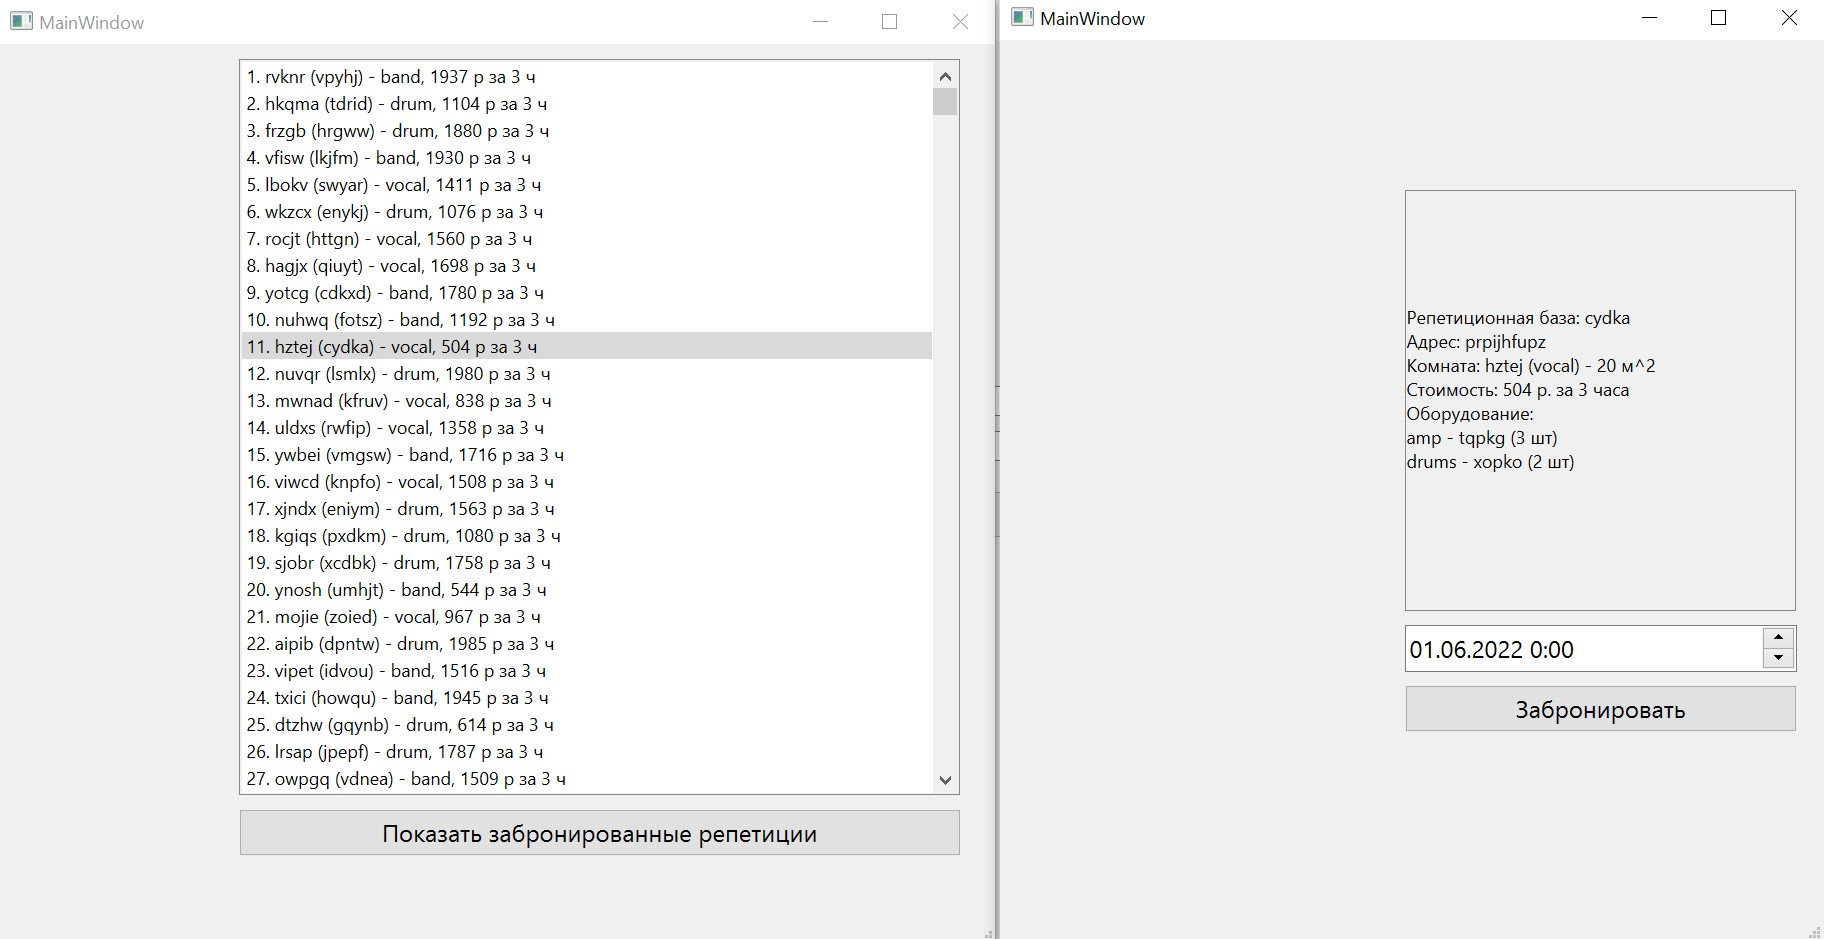
\includegraphics[scale=0.35]{jpg/Musician.jpg}
	\end{center}
	\captionsetup{justification=centering}
	\caption{Интерфейс при входе в качестве музыканта}
\end{figure}

\newpage

\begin{figure}[h!]
	\begin{center}
		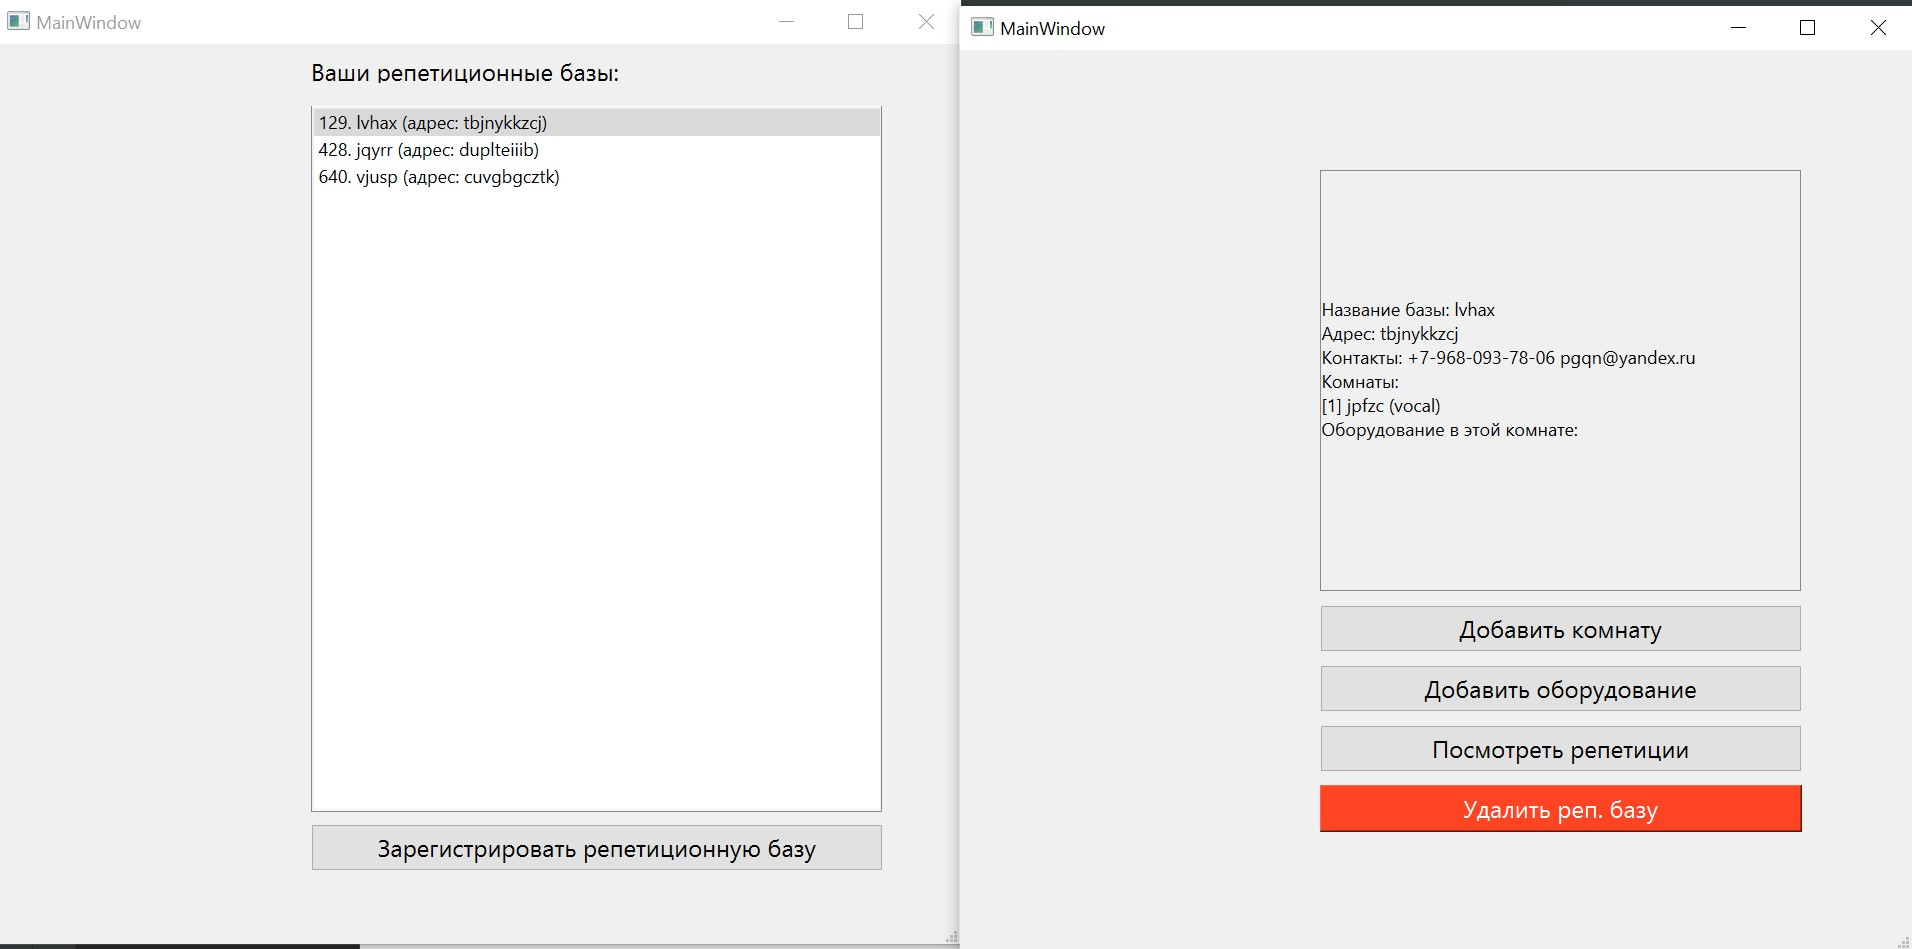
\includegraphics[scale=0.3]{jpg/Owner.jpg}
	\end{center}
	\captionsetup{justification=centering}
	\caption{Интерфейс при входе в качестве владельца}
\end{figure}

\begin{figure}[h!]
	\begin{center}
		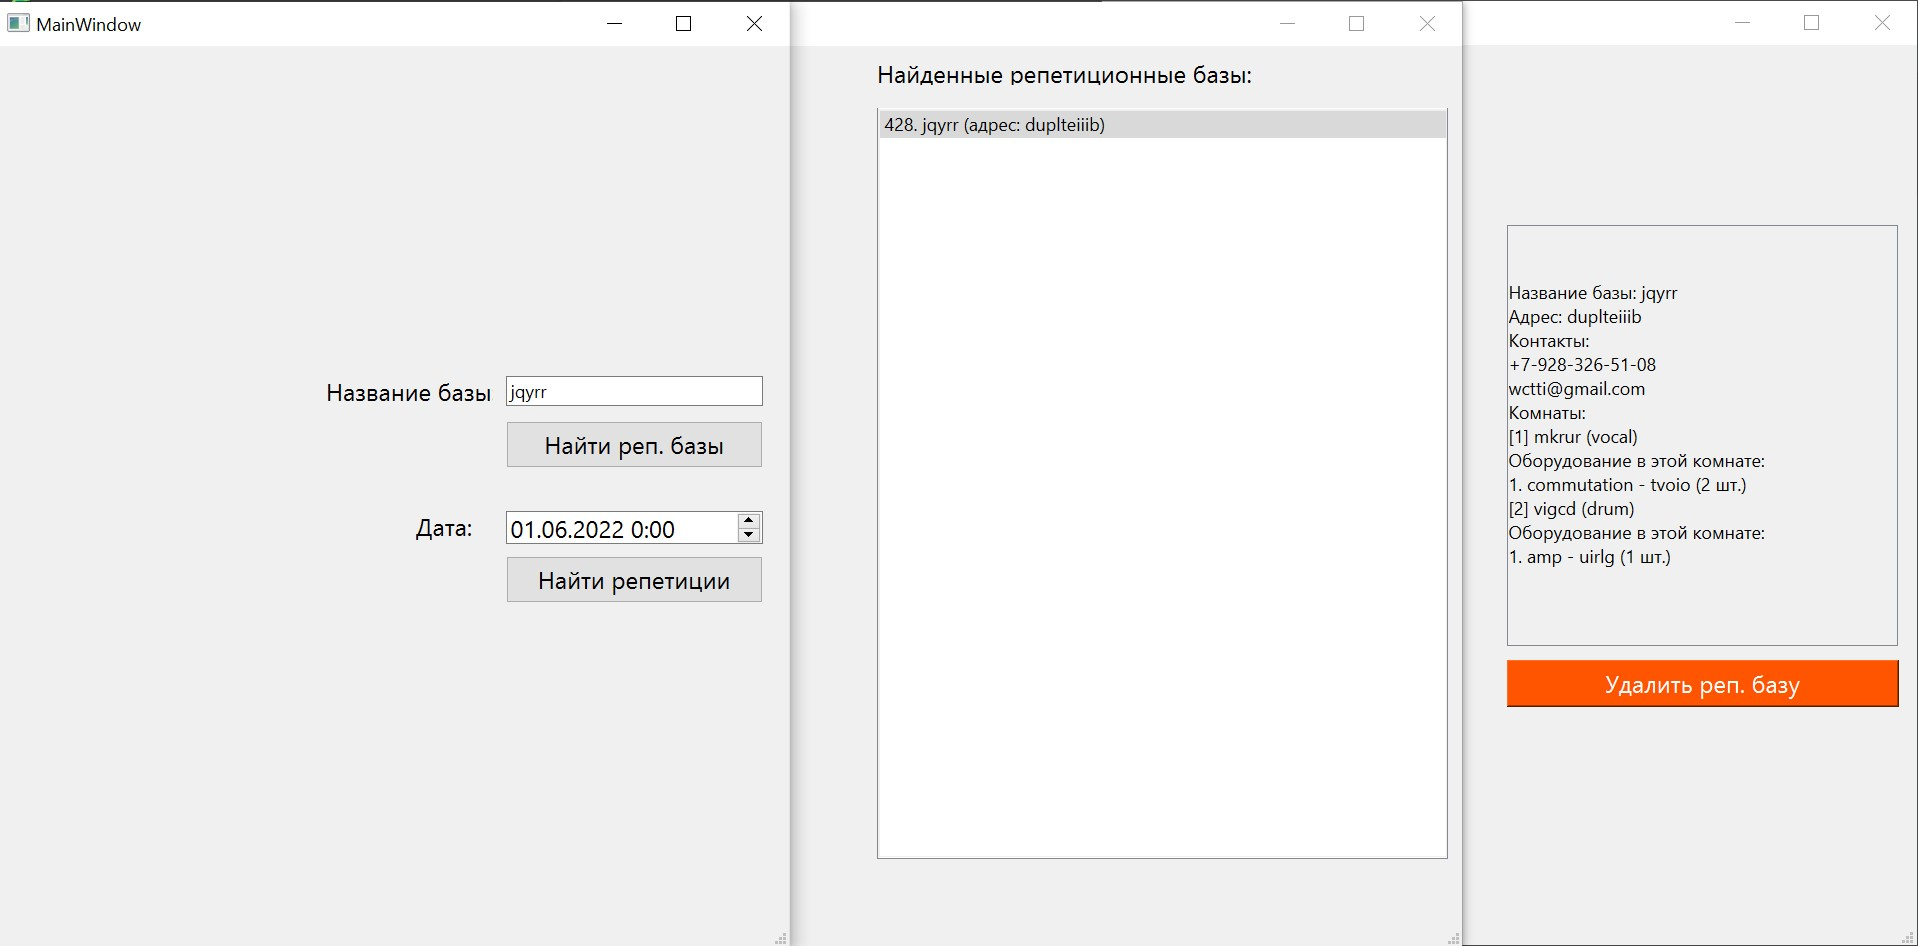
\includegraphics[scale=0.3]{jpg/Admin.jpg}
	\end{center}
	\captionsetup{justification=centering}
	\caption{Интерфейс при входе в качестве администратора}
\end{figure}

\newpage

\subsection*{Выводы}

В данном разделе были выбраны СУБД, язык программирования и среда разработки.

В качестве СУБД выбрана PostgreSQL, так как она:
\begin{itemize}
	\item свободно распространяемая;
	\item полностью соответствует требованиям ACID;
	\item поддерживает все необходимые в рамках поставленной задачи функции (такие, как вложенные селекты, транзакции, триггеры, процедуры).
\end{itemize}

В качестве языка программирования был выбран Python, так как он:
\begin{itemize}
	\item поддерживает работу с PostgreSQL;
	\item объектно-ориентированный;
	\item обладает необходимыми расширениями для работы с графическим интерфейсом.
\end{itemize}

В качестве среды разработки был выбран PyCharm, так как он:
\begin{itemize}
	\item имеет свободно распространяемую версию;
	\item содержит множество удобств для написания и отладки кода, а также для работы с СУБД.
\end{itemize}

Помимо этого, в данном разделе был разработан и протестирован исходный код программы. Программа тестировалась в соответствии с этапами, приведёнными в разделе 2.4. Все тесты были успешно пройдены.
